\newcommand {\To}{\rightarrow}
\newcommand {\TO}{\Rightarrow}
\newcommand {\R}{\mathbb{R}}
\newcommand {\Prob}{\mathbb{P}}
\newcommand{\E}{\mathbb{E}}
\newcommand {\cov}{\textrm{Cov}}
\newcommand {\var}{\textrm{Var}}
\newcommand {\1}{\textrm{\textbf{1}}}
\newcommand{\M}{\mathcal{M}}

\section{Abstract}\label{abstract}

The clustering and classification of functional data, discretely-sampled
curves varying over a continuum, is frequently encountered in machine
learning. While one can naively treat the data as vectors in Euclidean
space, one may also regard the data as functions. The challenge of
analyzing infinite-dimensional objects can be ameliorated if the curves
are smooth since the dimensionality is then only artificially high. This
insight underpins functional data analysis, a subfield of statistics
that studies functional data. For certain types of functional data such
as probability density functions and warped curves of a common template
function, there is further structure to exploit. Namely, certain
functional data may lie on a manifold of low intrinsic dimension. For
nonlinear manifolds, even basic operations such as addition and
subtraction require special consideration. This work addresses the
estimation of pairwise geodesic distances between noisy functional
manifold data that live near, rather than on, a manifold. This setting
cannot be tackled by classic manifold learning techniques which require
data to live exactly on a manifold. The proposed methodology first sends
the observed functional data to the hidden manifold, estimated using
subspace-constrained mean-shift. Geodesic distances are subsequently
calculated by employing shortest-path algorithms on this estimated
manifold. Improved estimation of the pairwise geodesic distance has
beneficial implications for many downstream tasks in functional data
analysis which we illustrate in the case of distance-based functional
classification/clustering.

\section{Introduction}\label{introduction}

Many statistical and machine learning methods rely on some measure of
distance. For example, clustering and classification of functional data,
discretely-sampled data varying over a continuum, is a common machine
learning task in which distance plays a crucial role. The successful
development of functional data analysis, a branch of statistics
dedicated to the analysis of infinite-dimensional smooth curves,
demonstrates that employing the \(L^2\) distance between the smoothed
functional observations has advantages over the Euclidean distance
between functional observations treated as vectors. In this work, we
advocate that for functional manifold data, i.e.~functional data that
lie on a manifold, the geodesic distance is potentially even better than
the \(L^2\) distance, with benefits realized in downstream tasks such as
distanced-based clustering and classification of functional manifold
data. In other words, when the manifold hypothesis is plausible,
e.g.~classes of probability density functions and classes of warped
curves of a common template function, clustering and classification
using the goedesic distance may give better results than using the
\(L_2\) distance.

Let \(X_1,\ldots,X_n\) be a sample of \(n\) independant realizations of
a random variable \(X\) that takes value in the Hilbert space
\(L^2([a,b],\R)\). Suppose additionally that the function \(X\) belongs
to a Riemannian manifold \(\M \subset L^2([a,b],\R)\) with Riemannian
metric tensor \(g\) which can be used to assign a metric on the manifold
as follows (Lin et al. 2014). For each point \(X\) on the manifold, the
Riemannian metric tensor \(g\) has an inner product \(g_X\) on the
tangent space \(T_X \M\). The norm of a tangent vector \(V \in T_X \M\)
is defined as \[||V|| = \sqrt{g_X(V,V)}.\] The geodesic distance between
two functions \(X_i,X_j\) on the manifold \(\M\), based on this metric
tensor \(g\), is defined as
\[ d_{\M}(X_i,X_j):=\inf \{l(\gamma): \gamma \text{ is piecewise-smooth function from } [a,b] \text{ to } \M, \gamma(a) = X_i, \gamma(b) = X_j \}\]
where \[ l(\gamma) := \int_a^b || \frac{\,d\gamma}{\,d t}(t) || \,dt\]
is the length of the curve \(\gamma\). ???Is it clear how \(l(\gamma)\)
depends on \(g\)???

Ideally, the functions \(X_i\) and \(X_j\) are observed on a very dense
domain grid with no measurement error. Then the estimation of the
geodesic distance \(d_\M(X_i,X_j)\) is straightfoward, e.g.~a
shortest-path algorithm such as Floyd-Warhsall (Floyd 1962) may be used.
However, most shortest-path algorithms critically assume observations
live on the manifold ???add reference??? and are thus likely to fail for
functional data which are almost certainly observed with noise. In this
work, we put forth a technique for the recovery of the \(n{\times}n\)
matrix \(G\) of pairwise geodesic distances, i.e.\\
\[
G(i,j)=G(j,i) = \begin{cases} 
      d_{\M} (X_i,X_j) & \textrm{if $i\neq j$,} \\
      0 & \textrm{otherwise.}
   \end{cases}
\] In lieu of \(X_i\) and \(X_j\), we have access only to
discretely-sampled noisy functional observations \(Y_i\) and \(Y_j\)
that possibly lie off the true manifold.

The work of (Chen and Muller 2012) was among the first in functional
data analysis to consider the manifold hypothesis for functional data. A
notion of the mean and variation of functional manifold data was
introduced there. Of particular relevance to this work is their proposed
P-ISOMAP procedure which adds a penalty to allow for noisy functional
observations whereas the classic ISOMAP algorithm (Tenenbaum, Silva, and
Langford 2000) assumes observations lie exactly on the manifold.
(Dimeglio et al. 2014) also realized this drawback to ISOMAP and
proposed a procedure we will call robust-ISOMAP that is less sensitive
to outliers. We will discuss P-ISOMAP and robust-ISOMAP in more details
in the simulation section.

\section{Proposed method for estimating geodesic
distances}\label{proposed-method-for-estimating-geodesic-distances}

Suppose that each curve \(X_i \in (\M,g)\) is observed with measurement
error on a time grid
\(T_i=(t_{i1},\ldots,t_{iK}), a \le t_{i1} < \ldots < t_{iK} \le b\),
i.e.~we observe a sample of \(K\)-dimensional vectors \(Y_1,\ldots,Y_n\)
with \(Y_{ij} = X_i(t_{ij}) + \epsilon_{ij}\), where the random
variables \(\epsilon_{ij}\) have mean zero and are uncorrelated with
each other. We assume that each observation grid \(T_1,\ldots,T_n\) is
dense, i.e.~\(K\) is large.

We begin by converting the discretly-sampled functional observations
into continuous ones. Let \(\tilde X_1,\ldots,\tilde X_n\) denote the
functional versions of the raw data obtained by some smoothing method.
For example, we may employ spline smoothing ???add reference for spline
smoothing??? to recover the functional versions of the raw data, i.e.\\

\begin{equation}\label{eq_spline_smoothing} 
\tilde X_i = \arg \min_{f\in C^2[0,1]}\left\{\sum_{j=1}^{K}\left(f(t_{ij})-Y_{ij}\right)^2+\lambda \|\partial^2_tf\|^2_{L^2}\right\},
\end{equation}

where \(\lambda>0\) is a tuning parameter controlling the smoothness of
\(\tilde X_i\). The proposed methodology for estimating the pairwise
geodesic distances \(\{ d_\M (X_i,X_j)\}_{i>j}\) is agnostic to the
smoothing method employed.

Our method is based on the idea that the underlying functional manifold
\(\M\) can be sufficiently well-recovered by the subspace-constrained
mean-shift (SCMS) algorithm (Ozertem and Erdogmus 2011). Let
\(\hat M \subset L^2([a,b],\mathbb R)\) denote the collection of basins
of attraction of the estimated probability density function of \(X\).
The SCMS algorithm sends each point
\(\tilde X_i \in L^2([a,b],\mathbb R)\) to a point in \(\hat M\). This
destination is unique and we denote it \(\tilde X_i^{\hat \M}\). We
expect the points
\(\tilde X^{\hat \M}_1,\ldots,\tilde X^{\hat \M}_n \in \hat M\) to lie
close to the real manifold \(\M\). Theoretical justificaton that
\(\hat M\) as estimated by SCMS is a reasonable surrogate for the true
manifold \(\M\) can be found in (Genovese et al. 2014).

Before presenting our procedure, we need to first review the ISOMAP
algorithm (Tenenbaum, Silva, and Langford 2000), a three-step procedure
that takes as input a set of points \(x_1,\ldots,x_n\) in a submanifold
\(\M\) of \(\R^D\) and produces an embedding in the space \(\R^d\) with
\(d<D\) that preserves pairwise geodesic distances. The procedure is as
follows.

\begin{enumerate}
\item Construct a weighted graph $G$ with nodes corresponding to the observations $x_1,\ldots,x_n\in \R^D$. Two nodes $x_i$ and $x_j$ are connected by an edge $e_{ij}$ with weight $d_{ij} 1\{d_{ij} \le \epsilon \}$ where $d_{ij}=||x_i-x_j ||_{2}$ and $\epsilon > 0$.
\item Estimate the pairwise geodesic distances $d_\M(x_i,x_j)$ based on $G$ using shortest-path algorithms. Specifically, the geodesic distance between two nodes is estimated to be the length of the shortest path in $G$ between these two nodes, i.e.\ the sum of the weights of the edges forming the shortest path, which is calculated either with the Floyd-Warshall algorithm [@Floyd1962] or with the Dijkstra algorithm [@Dijkstra59anote].
\item Use multidimensional scaling ???add reference??? to obtain an embedding in $\R^d$ that preserves the pairwise geodesic distances estimated above.
\end{enumerate}

Note that shortest-path algorithms such as the Floyd-Warshall algorithm
are used to find the smallest path \textit{given} a weigthed graph but
they do not produce the weighted graphs themselves. Both P-ISOMAP and
robust-ISOMAP are modifications of ISOMAP in the sense that they change
the construction of the weighted graph in step 1.\\

In what follows, we call IsoGeo the two-step procedure which performs a
modified version of the first step of ISOMAP followed by the original
second step of ISOMAP. The first step of IsoGeo constructs the weighted
graph \(G\) accoding to Dimeglio et al. (2014) so that graph is
independent of the tuning parameter \(\epsilon\). Specifically, we begin
by constructing the complete ???explain what complete means??? weighted
graph \(G_c\) with nodes corresponding to the observations
\(x_1,\ldots,x_n\in \R^D\). Next, we obtain the minimal spanning tree
associated with \(G_c\) and denote its set of edges by \(E_s\). The
graph \(G\) is obtained by adding all edges \(e_{ij}\) to \(E_s\) for
which the following condition is true:
\[ \overline{x_ix_j} \subset \bigcup_{i=1}^n B(x_i,\epsilon_i),\] where
\(B(x_i,\epsilon_i)\) is the open ball of center \(x_i\) and radius
\(\epsilon_i = \max_{e_{ij}\in E_s}d_{ij}\), and
\(\overline{x_ix_j}= \{x\in R^D \ | \ \exists \lambda \in [0,1], x=\lambda x_i + (1-\lambda)x_j \}\).
Let the distance estimated by IsoGeo be denoted
\(\text{IsoGeo}(x_i,x_j)\). Note that IsoGeo has no tuning parameters.

We are now ready to describe our procedure. Since SCMS is based on
kernel density estimation, we first reduce the dimension of our data
with multidimensional scaling before applying SCMS to avoid the curse of
dimensionality.

\begin{enumerate}
\item Discretise the functions $\tilde X_1,\ldots,\tilde X_n$ by evaluating them on a dense common grid $\tilde T=(t_{1},\ldots,t_{D})$. Let $s$ be a positive integer, much smaller than $D$. Obtain $\tilde X^s_1,\ldots,\tilde X^s_n \in \mathbb R^s$ using multidimensional scaling whereby the pairwise $\mathbb R^D$ Euclidean distances of the discretised functions $\tilde X_i$ are preserved.
\item Apply the subspace constrained mean-shift algorithm [@Ozertem2011] to each of $\tilde X^s_i$ to obtain $\tilde X^{s,\hat \M}_i$.
\item Use IsoGeo on the inputs $(\tilde X^{s,\hat \M}_1,\ldots,\tilde X^{s,\hat \M}_n)$ to obtain $\text{IsoGeo}(\tilde X^{s,\hat \M}_i,\tilde X^{s,\hat \M}_j)\}_{i>j}$.
\end{enumerate}

Our geodesic distance estimator is the \(n{\times}n\) matrix \(\hat G\)
whose elements are given by \[
\hat G(i,j)=\hat G(j,i) = \left\{ \begin{array}{ll}
 \text{IsoGeo}(\tilde X^{s,\hat \M}_i,\tilde X^{s,\hat \M}_j) & \textrm{if $i\neq j$,}\\
 0 & \textrm{otherwise.}
  \end{array} \right.
\]

There are two tuning parameters to our procedure. First, there is the
dimension \(s\) in step 1. In our simulations we try
\(s \in \{1,2,3\}\). The other parameter is the bandwidth \(h\) in the
subspace constrained mean-shift. In our simulations we set \(h\)
according to the heuristic in Equation (A1) of (Chen et al. 2015). In
reality, depending on the downstream task, both \(s\) and \(h\) can be
tuned in a data-adaptive way, say using cross-validation.

\section{Simulation study}\label{simulation-study}

We perform a simulation study to ascertain the efficacy of our method
for estimating pairwise geodesic distances. Three different metrics are
used to assess the quality of a pairwise geodesic distance estimator.

The first metric assesses near-\(\epsilon\) isometry, which we define as
the percentage of estimated pairwise geodesic distances between
\(1-\epsilon\) and \(1+\epsilon\) of the corresponding true pairwise
geodesic distance. We form the receiver operating curve with
\(\epsilon\) on the \(x\)-axis and near-\(\epsilon\) isometry on the
\(y\)-axis. The metric is the area under the receiver operating curve.

The second metric \(||d-\hat d||/||d||\) is the Frobenius norm of the
estimation error matrix \(d-\hat d\), relative to the Frobenius norm of
the true distance matrix \(d\). The third metric is the Pearson
correlation coefficient between the upper diagonal of \(d\) and
\(\hat d\).

\subsection{Alternative estimators of geodesic distance
{[}Marie{]}}\label{alternative-estimators-of-geodesic-distance-marie}

We compare the performance of our method to each of the following four
methods. The first method, denoted RD for raw data, takes the naive
approach of applying IsoGeo directly on the raw vectors
\(Y_1,\ldots,Y_n \in R^K\). Note that this procedure is only sensible if
all the grids \(T_1,\ldots,T_n\) are the same. In the second method, we
first smooth the discretely-sampled noisy functional data and then
estimate their pairwise distance using the \(L^2\) distance.

The third alternative, denoted SS for spline smoothing, applies IsoGeo
on the smoothed version \(\tilde X_1,\ldots,\tilde X_n\) of the raw data
obtained by spline smoothing as described in
(\ref{eq_spline_smoothing}). The final alternative we consider is
P-ISOMAP, denoted pI, which is the two-step procedure developed in Chen
and Muller (2012) designed to handle noisy functional data. In the first
step, a penalty is incorporated to robustify the construction of the
weighted graph. This is followed by the original second step of ISOMAP.

We ran Chen and Muller's P-ISOMAP separately in Matlab and tuned for the
number of neighbors and the penalty parameter using the relative
Frobenius assessment metric. We found that the penalty parameter chosen
in this way was always zero, thus reducing hte P-ISOMAP procedure to
standard ISOMAP. Given this, we did not make further comparison to
P-ISOMAP in our simulation study.

\subsection{Simulation scenarios}\label{simulation-scenarios}

We shall consider three functional manifolds in our simulation study. As
of yet, there is little work as to how to sample from a functional
manifold. Even in the Euclidean case, it is not obvious how sampling
should be done (Diaconis, Holmes, and Shahshahani 2013). How to properly
sample from a functional manifold could be interesting future work. For
now, to safeguard against sampling unevenly on the functional manifold,
we sample on a very concentrated measure for the intrinsic parameters.

\textbf{Isometric functional manifold of normal density functions} This
scenario is modified from what is referred to as Manifold 2 in (Chen and
Muller 2012) by fixing the variance of the normal density to be \(1\).
We have
\[\M =  \left \{X_\beta: \beta \in [-1,1], t \in [a,b]\right \}\] with
the \(L_2\) inner product as the metric tensor of \(\M\), where
\(X_\beta: [a,b] \to \R\) is given by
\(X_\beta(t) = \frac{1}{\sqrt{2\pi}} \exp{[-\frac{1}{2}(t-\beta)^2]}\).
First, note that the ``straight'' line connecting \(X_{\beta_1}\) and
\(X_{\beta_2}\) in \(\M\) does not always stay inside of \(\M\). Thus
the geodesic distance will not coincide with the \(L^2\) distance.

We set \(a=-4\) and \(b=4\) and sample \(\beta\) according to a
truncated standard normal with support on \([-1,1]\). The geodesic
distance between the curves \(X_{\beta_1}\) and \(X_{\beta_2}\) is given
by

\begin{eqnarray*}
d(X_{\beta_1},X_{\beta_2}) &=& \int_{\beta_1}^{\beta_2} \left \| \frac{d X_\beta (t)}{d\beta} \right\|_{L^2} d\beta \\
&=&  \int_{\beta_1}^{\beta_2} \sqrt{ \frac{1}{2\sqrt{\pi}} \int_{-4}^4 \frac{1}{\sqrt{\pi}} \exp\{-(t-\beta)^2\}(t-\beta)^2 dt  }  \  d\beta \\
&=&   \int_{\beta_1}^{\beta_2} \sqrt{ \frac{1}{2\sqrt{\pi}} \int_{-4}^4(t-\beta)^2 f(t) dt  }  \  d\beta, \textrm{ where $f$ is the density of a N$(\beta,1/2)$ }   \\
&\approx&  \int_{\beta_1}^{\beta_2}  \sqrt{ \frac{1}{2\sqrt{\pi}} \frac{1}{2}} \ d\beta \\
&=& (\beta_2-\beta_1) \frac{1}{2\pi^{1/4}},
\end{eqnarray*}

where the approximation comes from the fact that we are integrating on
\([a,b]=[-4,4]\) and not on \(\R\). We can see this manifold is
isometric, since the geodesic distance between \(X_{\beta_1}\) and
\(X_{\beta_2}\) in \(\M\) is proportional to \(\beta_2-\beta_1\), the
Euclidean distance between the \(\beta\)'s.

\textbf{Functional manifold of square root velocity functions} It was
shown in Joshi, Srivastava, and Jermyn (2007) that the square root
representation of probability density functions gives rise to a simple
closed-form geodesic distance. They consider the manifold
\[ \M = \{ \psi:[0,1] \to \R : \psi \ge 0, \int_0^1 \psi^2(s) \,ds = 1 \}\]
with the metric tensor given by the Fisher-Rao metric tensor
\[ <v_1,v_2> = \int_0^1 v_1(s) v_2(s) \,ds \] for two tangent vectors
\(v_1,v_2 \in T_\psi(\M)\). Note that this concides with the
\(L_2[0,1]\) inner product. Joshi, Srivastava, and Jermyn (2007) showed
that the geodesic distance between any two \(\psi_1\) and \(\psi_2\) in
\(\M\) is simply \[d_\M(\psi_1,\psi_2) = \cos^{-1}<\psi_1,\psi_2>.\] We
will specifically examine the square root of \(Beta(\alpha,\beta)\)
distributions which is supported on \([0,1]\). That is,
\[ M = \{ \psi_{\alpha,\beta}: 1 \le \alpha \le 5, 2 \le \beta \le 5\} \]
where \(\psi_{\alpha,\beta}: [0,1] \to \R\) is the pdf of
\(Beta(\alpha,\beta)\). We sample \(\alpha\) according to a truncated
normal with mean 3 and variance 0.09 with support on \([1,5]\). We
sample \(\beta\) according to a truncated normal with mean 3.5 and
variance 0.09 with support on \([2,5]\).

\textbf{Functional manifold of warping functions} This is based on
Equations 17 and 18 in Kneip and Ramsay (2008) but with
\(z_{i1}, z_{i2}\) both set to \(1\). (Note that Equation 17 has a typo
where the exponentials are missing negative signs.) Let
\(X_\alpha(t) = \mu(h_\alpha(t))\) be defined on \([-3,3]\) where
\[ \mu(t) = \exp\{(t-1.5)^2/2\} + \exp\{(t+1.5)^2/2\}\] and
\[ h_\alpha(t) = 6 \frac{ \exp\{\alpha(t+3)/6\} - 1}{\exp\{\alpha\}-1}\]
if \(\alpha \ne 0\) and \(h_\alpha(t) = t\) otherwise.

Consider the manifold \[ M = \{X_\alpha: -1 \le \alpha \le 1\}.\] We
sample \(\alpha\) according to a truncated standard normal with support
on \([-1,1]\). The geodesic distance is then
\[ d(X_{\alpha_1},X_{\alpha_2}) = \int_{\alpha_1}^{\alpha_2} \left \| \frac{d X_\alpha (t)}{d\alpha} \right\|_{L^2} d\alpha\]
which is estimated using numerical integration.

\subsection{Results}\label{results}

The tuning parameters for the proposed method were chosen as described
at the end of Section
\ref{proposed-method-for-estimating-geodesic-distances}. In step 1 of
our procedure, we take \(D = 100\) for the size of the common time grid.
We will investigate how two parameters affect the performance of the
various methods in consideration. The first one is the signal-to-noise
ratio ???describe??? which we fix at either \(0.1\) (low) or \(0.5\)
(high). The second parameter is \(K\), the dimension of the
dscrietly-observed noisy \(Y_i\)'s. We set \(K\) to either \(30\)
(sparse) or \(100\) (abundant).

We show the performance of the SS and L2 method versus our method for
three different values of \(s\). We omit the result of the square root
velocity scenario because all methods perform comparably. We can see
from Figures \ref{fig:normal} and \ref{fig:warping} that ???.

\begin{figure}
\centering
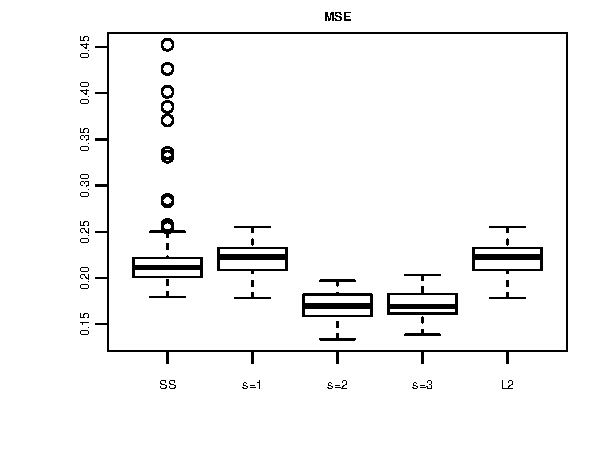
\includegraphics[height=0.3\textheight]{sim_results/sce=2_SNR=high_Kobs=30_MSE}
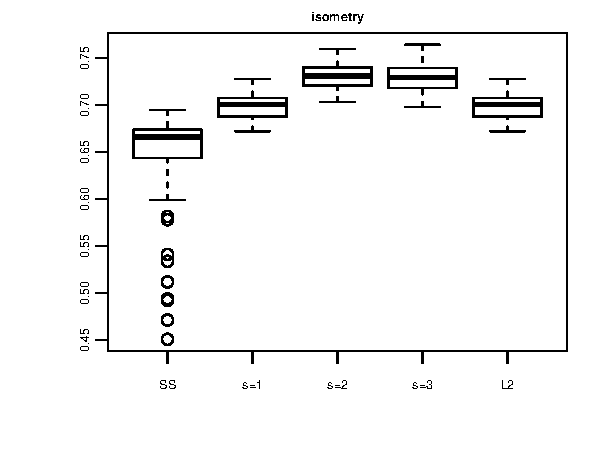
\includegraphics[height=0.3\textheight]{sim_results/sce=2_SNR=high_Kobs=30_isometry}
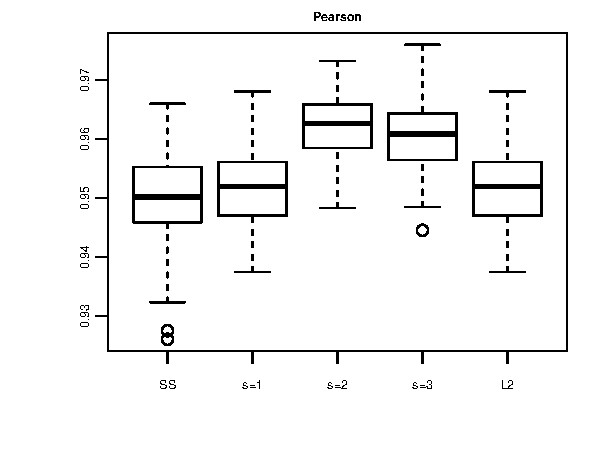
\includegraphics[height=0.3\textheight]{sim_results/sce=2_SNR=high_Kobs=30_Pearson}
\caption{Normal density}
\label{fig:normal}
\end{figure}

\begin{figure}
\centering
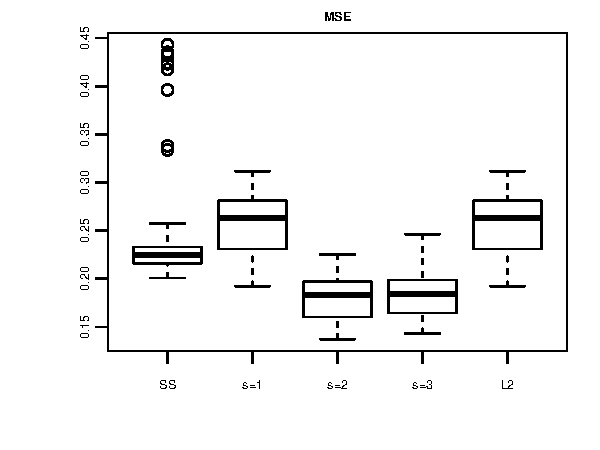
\includegraphics[height=0.3\textheight]{sim_results/sce=5_SNR=high_Kobs=30_MSE}
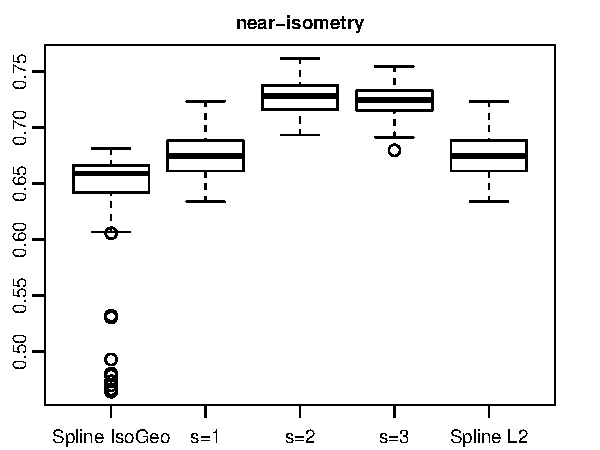
\includegraphics[height=0.3\textheight]{sim_results/sce=5_SNR=high_Kobs=30_isometry}
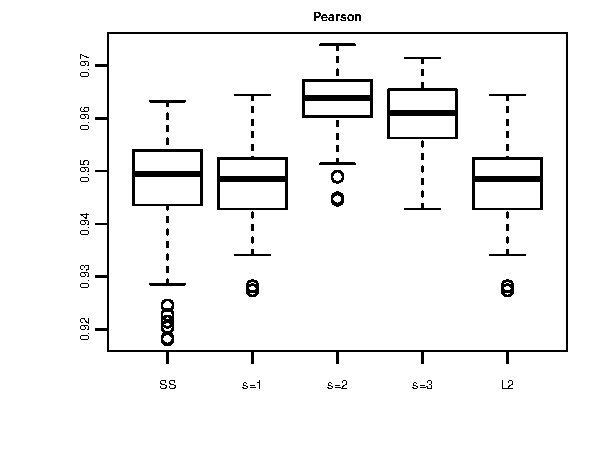
\includegraphics[height=0.3\textheight]{sim_results/sce=5_SNR=high_Kobs=30_Pearson}
\caption{Warping function}
\label{fig:warping}
\end{figure}

\section{Distance-based functional classification
{[}Marie{]}}\label{distance-based-functional-classification-marie}

In this section, we explore whether our geodesic distance estimator has
benefits for downstream analysis task. There are many tasks we could
consider here such as distance-based nonparametric regression and
distanced-based functional clustering, but we will focus on
distance-based functional classification. It must be noted that while
curve alignment, also known as curve registration, is necessarily
performed as a preprocessing technique prior to clustering and
classification, our geodesic distance estimator allows one to forsake
this step.

For simplicity, assume the task is binary classification. Associated to
each functional object \(x\) is a binary \(y\) indicating class
membership. Consider the classifier proposed in Ferraty and Vieu
(2003,2006) which is a functional version of the Nadaraya-Watson kernel
estimator of class membership probabilities: \[
\hat p(y = 0 | x) \frac{ \sum_{i=1}^n K[h^{-1} d(x,x_i)] 1(y_i = 0) }{ \sum_{i=1}^n K[h^{-1} d(x,x_i)] }
\] We shall compare our method to using \(L_2\) distance, possibly
weighted, and with curve registration already accomplished. Describe
alternative methods in detail.

The bandwidth in the classifier should be tuned individually for each
method. Also we might need to tune MDS dimension \(s\) since in real
data, the dimension of the manifold might be much higher than
encountered in the simulation scenarios where it never goes above 2.

Datasets used by functional classification papers

\begin{itemize}
\item Wheat, rainfall and phoneme in Aurore's paper "Achieving near-perfect classification for functional data"
\item Berkeley growth curves in [@ChenReiss2014].
\item Tecator and phoneme in [@Galeano2015] Mahalanobis technometrics paper.
\item yeast cell cycle gene expression (can't find this publicly) in [@LengMuller2005] "Classification using functional data analysis for temporal gene expression data"
\end{itemize}

Datasets used in functional manifold papers

\begin{itemize}
\item Berkeley growth, yeast cell cycle gene expression (can't find this publicly) in [@ChenMuller2012]
\item Tecator in [@LinYao2017] contamination paper
\item Berkeley growth, gait cycle in [@Dimeglio2014] robust isomap paper
\end{itemize}

\section*{References}\label{references}
\addcontentsline{toc}{section}{References}

\hypertarget{refs}{}
\hypertarget{ref-ChenMuller2012}{}
Chen, Dong, and Hans-Georg Muller. 2012. ``NONLINEAR Manifold
Representations for Functional Data.'' \emph{The Annals of Statistics}
40 (1). Institute of Mathematical Statistics: 1--29.
\url{http://www.jstor.org/stable/41713625}.

\hypertarget{ref-ChenHo2015}{}
Chen, Y., S. Ho, P. E. Freeman, C. R. Genovese, and L. Wasserman. 2015.
``Cosmic Web Reconstruction Through Density Ridges: Method and
Algorithm.'' \emph{Monthly Notices of the Royal Astronomical Society}
454 (1): 1140--56.
doi:\href{https://doi.org/10.1093/mnras/stv1996}{10.1093/mnras/stv1996}.

\hypertarget{ref-Diaconis2013}{}
Diaconis, Persi, Susan Holmes, and Mehrdad Shahshahani. 2013. ``Sampling
from a Manifold.'' In \emph{Advances in Modern Statistical Theory and
Applications: A Festschrift in Honor of Morris L. Eaton}, Volume
10:102--25. Collections. Beachwood, Ohio, USA: Institute of Mathematical
Statistics.
doi:\href{https://doi.org/10.1214/12-IMSCOLL1006}{10.1214/12-IMSCOLL1006}.

\hypertarget{ref-Dimeglio2014}{}
Dimeglio, Chloe, Santiago Gallon, Jean-Michel Loubes, and Elie Maza.
2014. ``A Robust Algorithm for Template Curve Estimation Based on
Manifold Embedding.'' \emph{Comput. Stat. Data Anal.} 70 (February).
Amsterdam, The Netherlands, The Netherlands: Elsevier Science Publishers
B. V.: 373--86.
doi:\href{https://doi.org/10.1016/j.csda.2013.09.030}{10.1016/j.csda.2013.09.030}.

\hypertarget{ref-Floyd1962}{}
Floyd, Robert W. 1962. ``Algorithm 97: Shortest Path.'' \emph{Commun.
ACM} 5 (6). New York, NY, USA: ACM: 345.
doi:\href{https://doi.org/10.1145/367766.368168}{10.1145/367766.368168}.

\hypertarget{ref-Genovese2014}{}
Genovese, Christopher R., Marco Perone-Pacifico, Isabella Verdinelli,
and Larry Wasserman. 2014. ``NONPARAMETRIC Ridge Estimation.'' \emph{The
Annals of Statistics} 42 (4). Institute of Mathematical Statistics:
1511--45. \url{http://www.jstor.org/stable/43556332}.

\hypertarget{ref-Joshi2007}{}
Joshi, S., A. Srivastava, and I.H. Jermyn. 2007. ``Riemannian Analysis
of Probability Density Functions with Applications in Vision.'' In
\emph{2007 Ieee Conference on Computer Vision and Pattern Recognition ;
Proceedings}, 1664--71. Piscataway, NJ: IEEE.
\url{http://dro.dur.ac.uk/18442/}.

\hypertarget{ref-Kneip2008}{}
Kneip, Alois, and James O Ramsay. 2008. ``Combining Registration and
Fitting for Functional Models.'' \emph{Journal of the American
Statistical Association} 103 (483). Taylor \& Francis: 1155--65.
doi:\href{https://doi.org/10.1198/016214508000000517}{10.1198/016214508000000517}.

\hypertarget{ref-Lin2014}{}
Lin, Binbin, Ji Yang, Xiaofei He, and Jieping Ye. 2014. ``Geodesic
Distance Function Learning via Heat Flow on Vector Fields.'' In
\emph{Proceedings of the 31st International Conference on International
Conference on Machine Learning - Volume 32}, II--145--II--153. ICML'14.
Beijing, China: JMLR.org.
\url{http://dl.acm.org/citation.cfm?id=3044805.3044909}.

\hypertarget{ref-Ozertem2011}{}
Ozertem, Umut, and Deniz Erdogmus. 2011. ``Locally Defined Principal
Curves and Surfaces.'' \emph{J. Mach. Learn. Res.} 12 (July). JMLR.org:
1249--86. \url{http://dl.acm.org/citation.cfm?id=1953048.2021041}.

\hypertarget{ref-Tenenbaum2000}{}
Tenenbaum, Joshua B., Vin de Silva, and John C. Langford. 2000. ``A
Global Geometric Framework for Nonlinear Dimensionality Reduction.''
\emph{Science} 290 (5500). American Association for the Advancement of
Science: 2319--23.
doi:\href{https://doi.org/10.1126/science.290.5500.2319}{10.1126/science.290.5500.2319}.
